%-*- coding: utf-8 -*-
\label{chap:nonlin}


\paragraph{Notions :} réseaux de neurones artificiels, apprentissage profond,
arbres de décision et forêts aléatoires, méthodes à noyaux.
\paragraph{Objectifs pédagogiques :} 
\begin{itemize}      
  \setlength{\itemsep}{3pt}
\item Décrire les similarités et différences entre réseaux de neurones artificiels et modèles linéaires ; 
\item Utiliser l'astuce du noyau pour apprendre des modèles non-linéaires à
  partir des algorithmes linéaires vus précédemment ;
\item Mettre en \oe{}uvre un algorithme d'apprentissage ensembliste.
\end{itemize}

Tous les modèles d'apprentissage supervisé que nous avons vus jusqu'à présent
utilisent une fonction linéaire des variables. Il s'agit dans ce chapitre
d'aborder comment construire des modèles non-linéaires, dont la capacité de
modélisation supérieure pourra permettre d'apprendre des modèles plus complexes. Attention néanmoins au surapprentissage !

Dans ce chapitre, nous considérons sauf mention contraire un jeu de données
$\DD = \{\xx^i, y^i\}_{i=1, \dots, n}$ de $n$ observations en $p$ dimensions et
leurs étiquettes dans $\YY$, avec $\YY= \{0, 1\}$ pour un problème de
classification binaire et $\YY = \RR$ pour un problème de régression.

\section{Modèles paramétriques non-linéaires}

\subsection{Régression polynomiale}
\label{sec:polynomial_reg}
Une première façon de construire des modèles non-linéaires, que nous avons
brièvement abordée dans la PC~4, consiste à apprendre une fonction de
décision de la forme suivante :
\begin{equation}
  \label{eq:polynomial_decision}
  f\colon \xx \mapsto \beta^0_0 + \sum_{j=1}^p \beta^1_{j} x_j + 
  \sum_{j=1}^p \sum_{k=1}^p \beta^2_{jk} x_j x_k + \dots +
  \underbrace{\sum_{j=1}^p \dots \sum_{\xi=1}^p}_{d \text{ termes}} \beta^d_{jk\dots\xi} x_j x_k \dots x_{\xi}.
\end{equation}
On parle alors de \textbf{régression polynomiale} de degré $d$.

Il s'agit en fait simplement d'une régression linéaire sur ${d+p \choose p}$ variables.

Attention, on crée ainsi un grand nombre de variables, corrélées entre elles :
il est alors indispensable d'utiliser un terme de régularisation pour éviter le
surapprentissage.

Le principe s'applique aussi à la régression logistique (vue dans la PC~5).


\subsection{Perceptron}
Les réseaux de neurones artificiels permettent d'autres formes de régressions
non-linéaires, et sont bien plus flexibles que les régressions polynomiales.


L'histoire des réseaux de neurones artificiels remonte aux années 1950 et aux
efforts de psychologues comme Franck Rosenblatt pour comprendre le cerveau
humain. Initialement, ils ont été conçus dans le but de modéliser
mathématiquement le traitement de l'information par les réseaux de neurones
biologiques qui se trouvent dans le cortex des mammifères. De nos jours, leur
réalisme biologique importe peu et c'est leur efficacité à modéliser des
relations complexes et non linéaires qui fait leur succès.
  
Le premier réseau de neurones artificiels est le \textbf{perceptron}, proposé
par Rosenblatt en 1957. Il comporte une seule couche et a une capacité de
modélisation limitée.
Le perceptron (figure~\ref{fig:perceptron}) est formé d'une couche d'entrée de
$p$ neurones, ou \textbf{unités}, correspondant chacune à une variable
d'entrée. Ces neurones transmettent la valeur de leur entrée à la couche
suivante.  À ces $p$ neurones on ajoute généralement une unité de biais, qui
transmet toujours la valeur $1$. Cette unité correspond à la colonne de $1$ que
nous avons ajoutée aux données dans les modèles linéaires
(équation~\eqref{eq:added_ones}). On remplacera dans cette section tout vecteur
$\xx = (x_1, x_2, \dots, x_p)$ par sa version augmentée d'un 1 :
$\xx = (1, x_1, x_2, \dots, x_p)$.

La première et unique couche du perceptron (après la couche d'entrée) contient
un seul neurone, auquel sont connectées toutes les unités de la couche
d'entrée.

Ce neurone calcule une combinaison linéaire
$o(\xx) = w_0 + \sum_{j=1}^p w_j x_j$ des signaux $x_1, x_2,  \dots, x_p$
qu'il reçoit en entrée, auquel il applique une \textbf{fonction d'activation}
$a$, dont il transmet en sortie le résultat. Cette sortie met en {\oe}uvre la
fonction de décision du perceptron.

Ainsi, si l'on appelle $w_j$ le poids de connexion entre l'unité d'entrée $j$
et le neurone de sortie, ce neurone calcule
\begin{equation}
  \label{eq:perceptron_sortie}
  f(\xx) = a(o(\xx)) = a\left(w_0 + \sum_{j=1}^p w_j x_j \right) 
  = a\left(\innerproduct{\ww,~\xx} \right).
\end{equation}
Il s'agit donc bien d'un modèle paramétrique.

\begin{figure}[h]
  \centering
  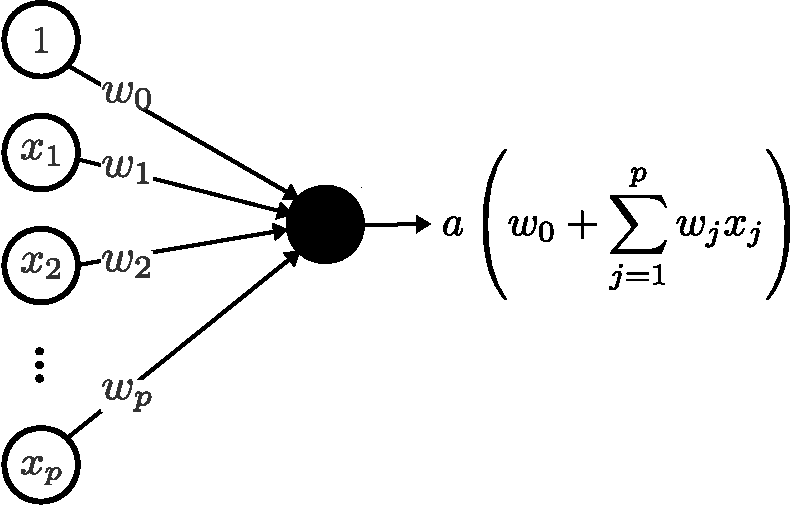
\includegraphics[width=0.5\textwidth]{figures/nonlin/perceptron}
  \caption{Architecture d'un perceptron. }
  \label{fig:perceptron}
\end{figure}

Dans le cas d'un problème de régression, on utilisera tout simplement l'identité comme fonction d'activation. Le modèle appris est donc $\xx \mapsto \innerproduct{\ww, \xx},$ comme dans le cas de la régression linéaire.

Le cas de la classification binaire, utilisant un seuil comme fonction
d'activation, est historiquement le premier à avoir été traité.  On utilisera
plutôt, comme dans le cas de la régression logistique (voir PC~5), une fonction
logistique (voir équation~\eqref{eq:sigmoide}) pour modéliser la probabilité
d'appartenir à la classe positive. Le modèle appris est donc
\begin{equation}
  \xx \mapsto \frac1{1 + e^{- o(\xx)}} = 
  \frac1{1 + \exp \left( - \innerproduct{\ww,~\xx} \right)}.
\end{equation}


\paragraph{Apprentissage incrémental} Pour entraîner un perceptron, nous
allons chercher, comme pour toute régresssion paramétrique, à minimiser le
risque empirique.  Cependant, nous allons supposer que les observations
$(\xx^i, y^i)$ ne sont pas disponibles simultanément, mais qu'elles sont
observées séquentiellement. Cette hypothèse découle de la plasticité des
réseaux de neurones biologiques : ils s'adaptent constamment en fonction des
signaux qu'ils reçoivent. Nous allons donc utiliser un algorithme
d'entraînement \textbf{incrémental}, qui s'adapte à des observations arrivant
les unes après les autres. En anglais, on parlera d'\textit{online
  learning}. Il s'agit donc d'appliquer un algorithme à directions de descente
itérativement, observation par observation, comme décrit dans la
section~\ref{sec:train_perceptron}, ou vous trouverez aussi plus de détails sur
les fonctions de perte utilisées. 
C'est cela qui distingue un perceptron d'une régression linéaire (pour la
régression) ou logistique (pour la classification).

\subsection{Entraînement du perceptron $\bullet$}
\label{sec:train_perceptron}

L'entraînement du perceptron commence par
une initialisation aléatoire du vecteur de poids de connexions
$\left( w_0^{(0)}, w_1^{(0)}, \dots, w_p^{(0)} \right)$, par exemple, $\ww = \vec{0}$.

Puis, à chaque observation, on ajuste ce vecteur dans la direction opposée au
gradient du risque empirique. Formellement, à une itération de l'algorithme,
on tire une nouvelle observation $(\xx^i, y^i)$ et on actualise, pour tout $j$,
les poids de connexion de la façon suivante :
\begin{equation}
  \label{eq:update_rule}
  w_j \leftarrow w_j - \eta \frac{\partial L(y^i, f(\xx^i))}{\partial w_j}.
\end{equation}

Il est possible (et même recommandé dans le cas où les données ne sont pas
extrêmement volumineuses) d'itérer plusieurs fois sur l'intégralité du jeu
de données. %Typiquement, on itère jusqu'à ce que l'algorithme converge à $\epsilon$ près.

Cet algorithme a un hyperparamètre, $\eta > 0$, qui est le pas de l'algorithme
du gradient et que l'on appelle la \textbf{vitesse d'apprentissage} (ou {\it
  learning rate}) dans le contexte des réseaux de neurones artificiels. Cet
hyperparamètre joue un rôle important : s'il est trop grand, l'algorithme
risque d'osciller autour de la solution optimale, voire de diverger. À
l'inverse, s'il est trop faible, l'algorithme va converger très lentement. Il
est donc essentiel de bien choisir sa vitesse d'apprentissage.

En pratique, on utilise souvent une vitesse d'apprentissage adaptative :
relativement grande au début, puis de plus en plus faible au fur et à mesure
que l'on se rapproche de la solution. Cette approche est à rapprocher
d'algorithmes similaires développés dans le cas général de l'algorithme du
gradient, comme par exemple la recherche linéaire par rebroussement
(\textit{backtracking line search}).

\paragraph{Classification probabiliste}
Dans le cas de la classification probabiliste, visant à prédire la probabilité
d'appartenir à la classe positive plutôt qu'une étiquette binaire, on utilise
l'entropie croisée comme fonction de coût (cf section~\ref{sec:cross_entropy}) :
\begin{equation*}
  L(y^i, f(\xx^i)) = 
- y^i \ln \left( \innerproduct{\ww,~\xx} \right) - (1-y^i) \ln \left( 1 - \innerproduct{\ww,~\xx}\right) 
\end{equation*}
Quelques lignes de calcul montrent que la règle d'actualisation~\eqref{eq:update_rule} devient :
\begin{equation}
  \label{eq:update_rule_class_prob}
  w_j \leftarrow w_j - \eta (f(\xx^i) - y^i) x_j^i.
\end{equation}

\paragraph{Régression}
Dans le cas de la régression, on utilise comme fonction de coût le
coût quadratique :
\begin{equation}
  L(y^i, f(\xx^i)) = 
  \frac12 \left(y^i - \innerproduct{\ww,~\xx}\right)^2.
\end{equation}
La règle d'actualisation~\eqref{eq:update_rule} devient :
\begin{equation}
  \label{eq:update_rule_reg}
  w_j \leftarrow w_j - \eta (f(\xx^i) - y^i) x_j^i.
\end{equation}
C'est exactement la même règle que pour la classification probabiliste (équation~\eqref{eq:update_rule_class_prob}).



\subsection{Perceptron multi-couche}
\label{sec:mlp}
La capacité de modélisation du perceptron est limitée car il s'agit d'un modèle
linéaire. Après l'enthousiasme généré par les premiers modèles connexionistes,
cette réalisation a été à l'origine d'un certain désenchantement au début des
années 1970... qui est maintenant bien loin derrière nous.
De l'annotation automatique d'images à la reconnaissance vocale, les récents
succès de l'intelligence artificielle sont nombreux à reposer sur les réseaux
de neurones profonds, et le {\it deep learning} (ou \textbf{apprentissage
  profond}) fait en effet beaucoup parler de lui.

On appelle \textbf{perceptron multi-couche}, ou {\it multi-layer perceptron}
({\it MLP}) en anglais, un réseau de neurones construit en insérant des
\textbf{couches intermédiaires} entre la couche d'entrée et celle de sortie
d'un perceptron. On parlera parfois de \textbf{couches cachées} par référence à
l'anglais {\it hidden layers}. Chaque neurone d'une couche intermédiaire ou de
la couche de sortie reçoit en entrée les sorties des neurones de la couche
précédente. Il n'y a pas de retour d'une couche vers une couche qui la précède
; on parle ainsi aussi d'un réseau de neurones \textbf{à propagation avant}, ou
{\it feed-forward} en anglais.
  
En utilisant des fonctions d'activation non linéaires, telles que la fonction
logistique, la fonction tangente hyperbolique, ou une fonction linéaire
seuillée (telle que ReLU, pour {\it Rectified Linear Unit}, qui dénote dans la
communauté de l'apprentissage profond la fonction $u \mapsto \max(0, u)$), on
crée ainsi un modèle paramétrique non linéaire.

\begin{exemple}
  Prenons l'exemple d'un perceptron avec deux couches intermédiaires comme
  illustré sur la figure~\ref{fig:mlp}. Notons $w^h_{jq}$ le poids de la
  connexion du neurone $j$ de la couche $(h-1)$ au neurone $q$ de la couche
  $h$, $a_h$ la fonction d'activation utilisée en sortie de la couche $h$,
  et $p_h$ le nombre de neurones dans la couche $h$.
  
  La sortie $z_q^1$ du $q$-ème neurone
  de la première couche cachée vaut
  % \begin{equation*}
    $z_q^1 = a_1\left(\sum_{j=0}^p w_{jq}^1 x_j \right).$
  % \end{equation*}
  La sortie $z_q^2$ du $q$-ème neurone de la deuxième couche cachée vaut
  % \begin{equation*}
    $z_q^2 = a_2\left(\sum_{j=1}^{p_1} w_{jq}^2 z_j^1 \right).$
  % \end{equation*}
  Enfin, la sortie du perceptron vaut
  % \begin{equation*}
    $f(\xx) = a_3\left(\sum_{j=1}^{p_2} w_{j}^3 z_j^2 \right).$
  % \end{equation*}
  
  Ainsi, en supposant qu'on utilise une fonction logistique pour tous les
  neurones des couches cachées, la sortie du perceptron vaut 
  \begin{equation*}
    f(\xx) = a_3\left(\sum_{j=0}^{p_2} w_{jq}^3 \frac1{1 + 
        \exp\left(- \sum_{j=0}^{p_1} w_{jq}^2 \frac1{1 + 
            \exp\left(- \sum_{j=0}^p w_{jq}^1 x_j \right)} \right)} \right),
  \end{equation*}
  ce qui devrait vous convaincre de la capacité du perceptron multi-couche à
  modéliser des fonctions non linéaires.
\end{exemple}
  
\begin{figure}[h]
  \centering
  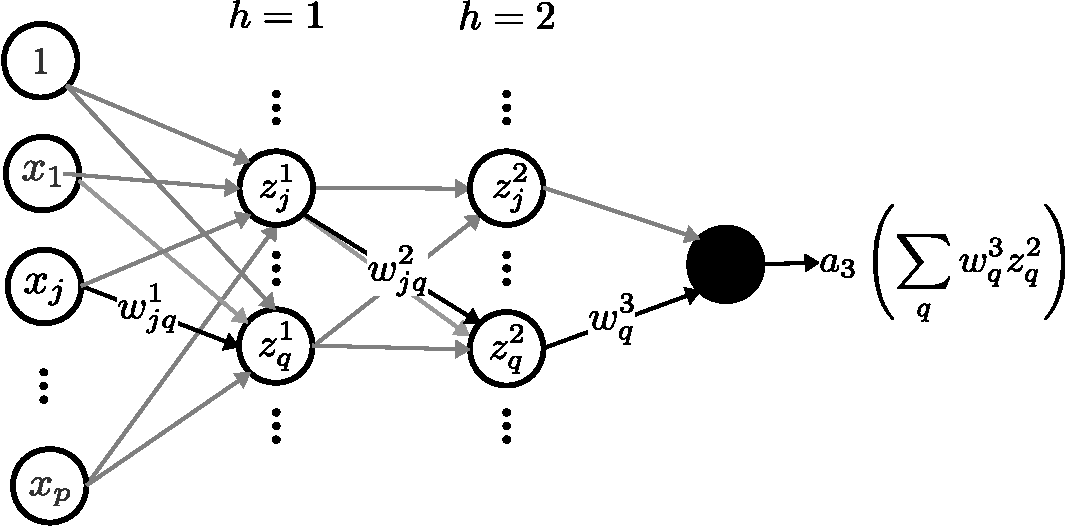
\includegraphics[width=0.8\textwidth]{figures/nonlin/mlp}
  \caption{Architecture d'un perceptron multi-couche. }
  \label{fig:mlp}
\end{figure}

\paragraph{Nombre de paramètres} Le perceptron multi-couche est un modèle
paramétrique dont les paramètres sont les poids de connexions $w_{jq}^h$. Le
nombre de couches et leurs nombres de neurones font partie des hyperparamètres
: on les suppose fixés, ce ne sont pas eux que l'on apprend. Ce modèle a donc
d'autant plus de paramètres (c'est-à-dire de poids de connexion) qu'il y a de
couches intermédiaires et de neurones dans ces couches. Cela leur confère une
grande puissance de modélisation (voir plus de détails à la
section~\ref{sec:universal_approx}), mais le risque de surapprentissage est
élevé.  Les réseaux de neurones profonds requièrent ainsi souvent des quantités
massives de données pour apprendre de bons modèles.

\subsection{Entraînement d'un perceptron multi-couche}
Il est important de remarquer que la minimisation du risque empirique pour un
perceptron multi-couche n'est {\it pas} un problème d'optimisation
convexe. Ainsi, nous n'avons pas d'autres choix que d'utiliser un algorithme à
directions de descente, sans aucune garantie de converger vers un minimum
global.

L'initialisation des poids de connexion, la standardisation des variables, le
choix de la vitesse d'apprentissage et celui des fonctions d'activation ont
tous un impact sur la capacité du perceptron multi-couche à converger vers une
bonne solution. Entraîner un réseau de neurones multi-couche n'est pas chose
aisée.

\paragraph{Rétropropagation} Néanmoins, le principe fondamental de
l'apprentissage d'un perceptron multi-couche, connu sous le nom de
\textbf{rétropropagation} ou {\it backpropagation} (souvent raccourci en {\it
  backprop}), est connu depuis des décennies. Il repose, comme pour le
perceptron, sur l'utilisation de l'algorithme du
gradient pour minimiser, à chaque nouvelle observation, le risque
$L(y^i, f(\xx^i))$. Pour plus de détails, reportez-vous à la
section~\ref{sec:backprop}.
  
\subsection{Deep learning}
Le domaine de l'\textbf{apprentissage profond} repose
fondamentalement sur les principes que nous venons de voir. En effet, un
perceptron multi-couche est profond dès lors qu'il contient suffisamment de
couches -- la définition de \og suffisamment \fg~étant subjective.  Le
domaine de l'apprentissage profond s'intéresse aussi à de nombreuses autres
architectures comme les \textbf{réseaux récurrents} ({\it RNN}, pour {\it
  Recursive Neural Nets}), et en particulier {\it Long Short-Term Memory (LSTM)
  networks} pour modéliser des données séquentielles (telles que du texte ou
des données temporelles) et les \textbf{réseaux convolutionnels} ({\it CNN},
pour {\it Convolutional Neural Nets}) pour le traitement d'images.

Dans tous les cas, il s'agit essentiellement d'utiliser ces architectures pour
créer des modèles paramétriques (potentiellement très complexes), puis d'en
apprendre les poids par un algorithme à directions de descente.

L'apprentissage des poids de connexion d'un réseau de neurones profond pose des
difficultés techniques : en effet, le problème d'optimisation à résoudre n'est
pas convexe, et il n'est pas évident de converger vers un « bon »
minimum. Cette tâche est d'autant plus difficile que le réseau est complexe, et
les progrès dans ce domaine ne sont possibles que grâce au développement de
méthodes pour la rendre plus aisée.

Une des techniques les plus importantes dans ce domaine est le
\textbf{pré-entraînement}, ou \textit{pretraining} : il s'agit d'utiliser un
réseau de neurones profond entraîné sur une très grosse base de données de même
nature que le problème que l'on cherche à résoudre pour initialiser
l'optimisation sur notre jeu de données. Par exemple, pour une tâche de
classification sur un jeu de données de quelques milliers d'images médicales,
on partira d'un réseau de neurones entraîné sur une base de données d'images
naturelles telle que ImageNet, qui contient des millions d'images appartenant à
plus de 20\,000 classes.

De plus, les réseaux de neurones profonds ont de nombreux paramètres, et
requièrent donc l'utilisation de grands volumes de données pour éviter le
sur-apprentissage. Il est donc généralement nécessaire de les déployer sur des
architectures distribuées.

Ainsi, malgré son succès dans certains domaines d'application (notamment
images, texte, et séries temporelles), le \textit{deep learning} est délicat à
mettre en place et n'est pas toujours la meilleure solution pour résoudre un
problème de \textit{machine learning}, en particulier face à un petit jeu de
données.

\paragraph{Apprentissage de représentations $\bullet$}
On associe souvent aux réseaux de neurones profond la notion de {\it
  representation learning}. En effet, il est possible de considérer que chacune
des couches intermédiaires successives apprend une nouvelle représentation
$(z^h_1, z^h_2, \dots, z^h_{p_h})$ des données à partir de la représentation de
la couche précédente, et ce jusqu'à pouvoir appliquer un algorithme linéaire à
la représentation contenue dans la dernière couche intermédiaire.


\section{Méthodes à noyaux}
Les méthodes à noyaux permettent de construire des modèles non-linéaires de
régression ou de classification sur le même modèle que la régression
polynomiale, mais sans avoir à calculer explicitement les nouvelles variables. 
Nous allons tout d'abord illustrer leur principe sur l'exemple de la régression ridge.

\subsection{Exemple de la régression ridge quadratique}

Nous utilisons ici les mêmes notations qu'à la section~\ref{sec:ridge_regression}.
La fonction de prédiction de la régression ridge est de la forme
% \begin{equation}
%   \label{eq:reg_ridge_pred}
  $f\colon \xx \mapsto \langle \xx,  \bbeta^* \rangle,$
% \end{equation}
où $\bbeta^*$ est donné par l'équation~\eqref{eq:ridgereg_sol} :
\begin{equation}
  \label{eq:reg_ridge_beta}
  \bbeta^* =  \left( \lambda I_p + X^\top X  \right)^{-1} X^\top \yy.
\end{equation}
  
En remplaçant $\bbeta^*$ par sa valeur, la fonction de prédiction peut se réécrire comme :
\begin{equation}
  \label{eq:reg_ridge_2}
  f\colon \xx \mapsto \xx X^\top (\lambda I_n + XX^\top)^{-1} y.
\end{equation}
Vous en trouverez la preuve section~\ref{sec:ridge_rewrite}.


Nous allons maintenant traiter l'exemple de la \textbf{régression ridge
  quadratique}, c'est-à-dire d'une régression polynomiale de degré 2
régularisée par un terme $\ell_2$. 
Définissons l'application
\begin{equation*}
  \begin{split}
    \phi\colon \RR^p  & \to \RR^m \\
    (x_1, x_2, \dots, x_p) & \mapsto (1, \sqrt{2}\,x_1, \sqrt{2}\, x_2, \dots,
    \sqrt{2}\, x_p,~x_1^2, x_1 x_2, \dots, x_p^2),
  \end{split}
\end{equation*}
avec $m = 1+ p + \frac12 p(p+1)$ le nombre de monomes de $p$ variables de degré
au plus $2$.  Les coefficients $\sqrt{2}$ sont introduits ici pour des
facilités de calcul plus tard ; ils ne changent rien conceptuellement.

La fonction de décision d'une régression quadratique est une fonction
\textit{linéaire} de $\phi(\xx)$ : la régression polynomiale est équivalente à
une régression linéaire sur un espace de plus grande dimension (ici, $m$).  
Pour entraîner une régresion ridge quadratique, nous pouvons donc entraîner une
régression ridge sur les données $\{(\phi(\xx^1), y^1), (\phi(\xx^2), y^2), \dots, (\phi(\xx^n), y^n)\}.$

Posons donc $\Phi \in \RR^{n \times m}$ la matrice
décrivant les images des observations $(\xx^1, \xx^2, \dots, \xx^n)$ par $\phi$.
L'équation~\eqref{eq:reg_ridge_2}, appliquée à $\phi(\xx)$, devient alors
\begin{equation}
  \label{eq:reg_ridge_phi}
  f_\phi\colon \xx \mapsto \phi(\xx) \Phi^\top (\lambda I_n + \Phi \Phi^\top)^{-1} y.
\end{equation}

Définissons maintenant la fonction
\begin{equation}
  \label{eq:kernel}
  \begin{split}
    k \colon \RR^p \times \RR^p & \to \RR \\
    \xx,~\xx^\prime & \mapsto \innerproduct{\phi(\xx),~\phi(\xx^\prime)}.
  \end{split}
\end{equation}

Construisons le vecteur $\kappa \in \RR^n$ dont la
$i$-ème entrée est
  $\kappa_i = \innerproduct{\phi(\xx),~\phi(\xx^i)} = k(\xx, \xx^i)$,
et la matrice $K \in \RR^{n \times n}$ dont l'entrée $K_{il}$ est
$K_{il} = \innerproduct{\phi(\xx^i),~\phi(\xx^l)} = k(\xx^i, \xx^l).$
Nous pouvons maintenant réécrire l'équation~\eqref{eq:reg_ridge_phi} comme
\begin{equation}
  \label{eq:reg_ridge_k}
  f_\phi \xx \mapsto  \kappa (\lambda I_n + K)^{-1} y,
\end{equation}
dans laquelle $\phi$ n'apparait plus qu'à travers des produits scalaires (calcul de $\kappa$
et $K$).
Cela signifie que nous pouvons apprendre une régression ridge quadratique sans utiliser $\phi$, à condition de connaître $k$.

Cette phrase peut paraître surprenante, car nous avons défini $k$ en utilisant $\phi$.

Cependant, pour tout $\xx$ et $\xx^\prime$ de $\RR^p$,
\begin{equation*}
  k(\xx,~\xx^\prime) = \left(\innerproduct{\xx,~\xx^\prime} + 1 \right)^2.
\end{equation*}

Il est donc possible d'apprendre une régression ridge quadratique sans calculer
explicitement les images des $\xx^i$ ou de l'observation $\xx$ à étiqueter dans
$\RR^m$.

Cela a un intérêt calculatoire. En effet, calculer $\phi(\xx)$ puis
$\phi(\xx^\prime)$ puis leur produit scalaire requiert de l'ordre de
$2m + 2m = 2 + 2p + p(p+1)$ opérations. À l'inverse, calculer
$\innerproduct{\xx,~\xx^\prime}$ puis ajouter 1 et élever le tout au carré
requiert $p+2$ opérations : la deuxième option est moins coûteuse. Évidemment,
pour une régression quadratique et un faible nombre de variables, ces deux
valeurs sont toutes les deux faibles. Cependant, la différence de temps de calcul entre les deux approches va augmenter avec le nombre de variables et le degré de polynôme considéré.

La démarche que nous avons présentée ici se généralise à
\begin{itemize}
\item n'importe quelle fonction $k$ de deux variables s'écrivant sous la forme
  du produit scalaire des images de ces variables dans un espace de
  Hilbert\footnote{À savoir, un espace de dimension potentiellement infinie et
    muni d'un produit scalaire ; il s'agit d'une généralisation des espaces
    euclidiens. Vous pouvez considérer qu'un espace de Hilbert est $\RR^m$ ou
    $\mathbb{C}^m$, avec potentiellement « $m = +\infty$ ».} ;
\item n'importe quelle procédure d'apprentissage dans laquelle les observations
  n'apparaissent que sous la forme de produits scalaires entre observations.
\end{itemize}
C'est ce que nous faisons dans la section suivante.

\subsection{Méthodes à noyau}
\label{sec:kernels}

\paragraph{Noyau} On appelle \textbf{noyau} sur un espace quelconque $\XX$ toute
fonction $k\colon \XX \to \RR$ continue, symétrique et semi-définie
positive\footnote{au sens où
pour tout $N \in \NN$, pour tout $(\xx^1, \xx^2, \dots \xx^N) \in
  \mathcal{X}^N$ et pour tout $(a_1, a_2, \dots a_N) \in \RR^N$, 
  $\sum_{i=1}^N \sum_{l=1}^N a_i a_l k(\xx^i, \xx^l) \geq 0$. En particulier, la matrice $K$ définie à la section précédente est ainsi semi-définie positive.}.\\
Le \textbf{théorème de Moore-Aronszajn}\footnote{Démontré dans \textit{Theory
    of reproducing kernels}, N. Aronszajn, Transactions of the American
  Mathematical Society 68(3):337--40 (1950), et attribué à E. Hastings Moore.}
garantit alors l'existence d'un espace de Hilbert $\HH$ et d'une application
$\phi\colon \XX \to \HH$ telle que pour tout
$(\xx, \xx^\prime) \in \XX \times \XX,$
$k(\xx,~\xx^\prime) = \innerproduct{\phi(\xx),~\phi(\xx^\prime)}_\HH.$\\
Nous
appellerons $\HH$ l'\textbf{espace de redescription}, car il permet de décrire les éléments de $\XX$ avec de nouvelles variables.

\paragraph{Astuce du noyau} Étant donnée une procédure d'apprentissage
automatique dans laquelle les observations n'apparaissent que dans des produits
scalaires entre observations, on peut remplacer tous les produits scalaires en
question par un noyau. Cela revient à appliquer la même procédure
d'apprentissage dans l'espace de redescription.\\
Cela signifie que nous n'avons pas besoin de faire de calculs dans $\HH$, qui
est généralement de très grande dimension : c'est ce que l'on appelle
\textbf{l'astuce du noyau.} Elle s'applique non seulement à la régression
ridge, mais aussi à de nombreux autres algorithmes d'apprentissage, dont la SVM
(vues dans la PC~5), ce que vous pouvez lire en plus de détails dans la
section~\ref{sec:kernel_svm}.

Quand on applique l'astuce du noyau à la régression ridge, on parle de
\textbf{régression ridge à noyau} ou \textit{kernel ridge regression (KRR)} en
anglais.


Le \textbf{noyau polynomial} de degré $d \in \NN$,
défini sur $\RR^p \times \RR^p$ par
$k(\xx, \xx^\prime) = \left( \langle \xx, \xx^\prime \rangle + c\right)^d,$ où $c \in \RR$
permet d'inclure des termes de degré inférieur à $d$, correspond à un espace de
redescription $\HH$ comptant autant de dimensions qu'il existe de monômes de
$p$ variables de degré inférieur ou égal à $d$, soit $p+d \choose d$.

Encore plus puissant, le \textbf{noyau radial gaussien}, ou {\it noyau RBF}
(pour {\it Radial Basis Function}), de bande passante $\sigma > 0,$ et défini
sur $\RR^p \times \RR^p$ par
$k(\xx, \xx^\prime) = \exp\left( - \frac{||\xx - \xx^\prime||^2}{2 \sigma^2}
\right),$ correspond à un espace de redescription $\HH$ de dimension {\it
  infinie}, ce qui se démontre en utilisant le développement en série entière
de la fonction exponentielle (voir détails section~\ref{sec:rbf_kernel}).Ainsi,
l'équation~\eqref{eq:reg_ridge_k} où $\kappa$ et $K$ ont été calculés avec le
noyau RBF ci-dessus permet d'apprendre une régression polynomiale de degré
arbitrairement grand.

Vous trouverez plus d'exemples de noyaux dans la section~\ref{sec:more_kernels}.


\section{Arbres et forêts}
À l'exception de l'algorithme des $k$ plus proches voisins (cf. Projet numérique), les
algorithmes d'apprentissage supervisé que nous avons vus jusqu'à présent
permettent d'apprendre des modèles paramétriques. Les arbres de décision sont
un autre exemple de modèle simple et non-paramétrique \footnote{Les modèles
  appris par des méthodes à noyau sont aussi non-paramétriques : il n'y a plus
  d'hypothèse sur la distribution de $(X, Y)$. La complexité d'un modèle à
  noyau augmente avec le nombre d'observations.}.

\subsection{Arbres de décision}
On appelle \textbf{arbre de décision} (\textit{decision tree} en anglais) un
modèle prédictif qui peut être représenté sous la forme d'un arbre. Chaque
n{\oe}ud de l'arbre teste une condition sur une variable et chacun de ses
enfants correspond à une réponse possible à cette condition. Les feuilles de
l'arbre correspondent à une étiquette.

Pour prédire l'étiquette d'une observation, on \og suit \fg~les réponses aux
tests depuis la racine de l'arbre, et on retourne l'étiquette de la feuille à
laquelle on arrive.

Ils sont couramment utilisés en dehors du monde du machine learning, par
exemple pour décrire les étapes d'un diagnostic ou d'un choix de traitement
pour un médecin, ou les chemins possibles dans un \og livre dont vous êtes le
héros \fg. La figure~\ref{fig:fruit_tree} présente un tel arbre de décision.

Les arbres de décision permettent de traiter naturellement des variables
qualitatives. 
Ils permettent aussi de traiter des classes
multi-modales (comme ici pour l'étiquette \og pomme \fg, qui est affectée à un
fruit grand et rouge ou à un fruit jaune et rond.)


\begin{figure}[h]
  \centering
  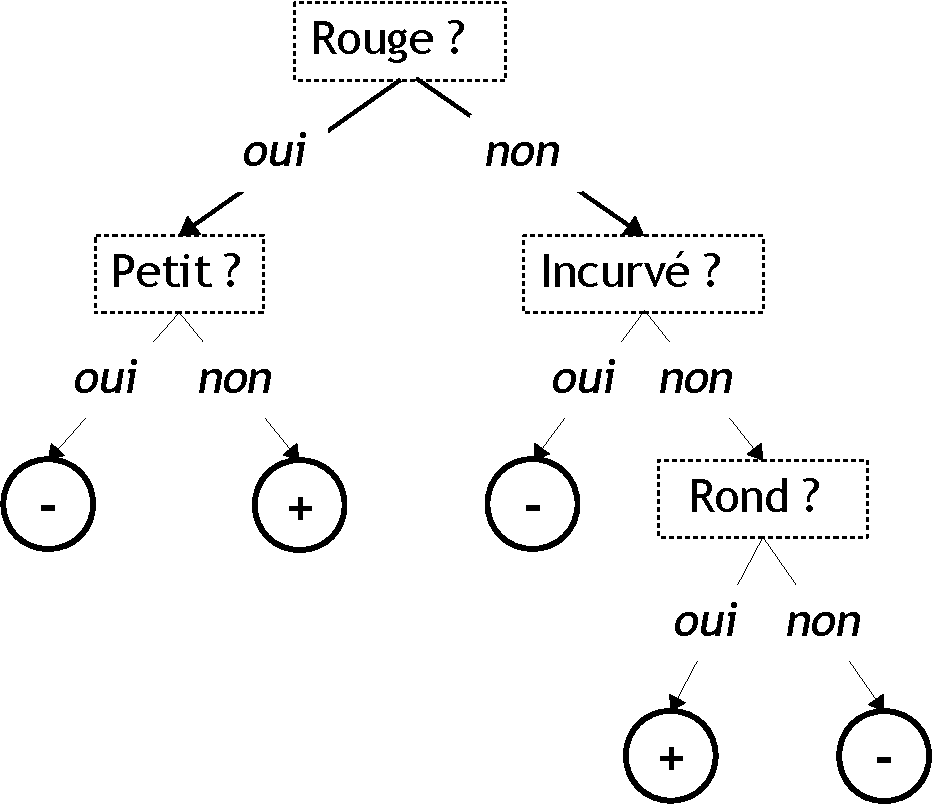
\includegraphics[width=0.5\textwidth]{figures/nonlin/fruit_tree}
  \caption{Exemple d'arbre de décision pour classifier des fruits entre pommes
    (+) et autres (-).}
  \label{fig:fruit_tree}
\end{figure}



\subsection{Comment faire pousser un arbre de décision (cas binaire)}
\label{sec:grow_tree_binary}
L'algorithme utilisé pour entraîner un arbre de décision est appelé
\textbf{CART}, pour {\it Classification And Regression Tree}. Il s'agit d'un
algorithme de partitionnement de l'espace par une approche gloutonne, récursive
et divisive.
Dans cette section, nous expliquons comment entraîner un arbre de décision pour
un problème de classification binaire sur des variables binaires : on considère
$\YY = \{0, 1\}$ et $x_j \in \{0, 1\}$ pour tout $j=1, \dots, p$. 

À chaque n{\oe}ud d'un arbre de décision construit par CART correspond une
\textbf{variable séparatrice} ({\it splitting variable})
$j \in \{1, \dots, p\}$ selon laquelle vont être partitionnées les
données. Cette variable séparatrice définit deux régions, correspondant aux
enfants du n{\oe}ud considéré :
\begin{equation*}
  R_l(j) = \{\xx~|~x_j = 0\} ; \hspace{2em} 
  R_r(j) =  \{\xx~|~x_j = 1\}.
\end{equation*}
Au niveau de la racine de l'arbre, $R_l$ et $R_r$ partitionnent l'ensemble des
observations. Ensuite, chaque n{\oe}ud partitionne uniquement les observations
qui sont arrivées jusqu'à lui, autrement dit qui vérifient toutes les
conditions dictées par ses parents. 

\paragraph{Exemple} Sur l'exemple de la figure~\ref{fig:fruit_tree}, au
n{\oe}ud « incurvé », $R_l$ est l'ensemble des fruits non rouge et de forme
incurvée, et $R_r$ est l'ensemble des fruits non rouge et de forme non incurvée. Si
la majorité des individus de $R_l$ ne sont pas des pommes, on associe alors
l'étiquette négative à tous les individus de $R_l$. Si la majorité des
individus de $R_r$ sont des pommes, on associe alors l'étiquette positive à
tous les individus de $R_r$ (malgré la présence de citrons dans $R_r$, qui ne
seront identifiés qu'au n{\oe}ud suivant).

À chaque itération de CART, on itère sur toutes les valeurs possibles de $j$
pour déterminer celle qui minimise localement l'erreur faite en attribuant à
toutes les observations d'une région l'étiquette majoritaire dans cette région.
Il s'agit donc bien d'un problème de minimisation du risque
empirique. Cependant, il s'agit d'un algorithme glouton : il n'y a aucune
garantie que cette stratégie aboutisse à l'arbre de décision dont l'erreur sur
le jeu d'entraînement est minimale.

\paragraph{Formalisation $\bullet$} On peut formellement noter :
\begin{equation}
  \argmin_{j \in \{1, \dots, p\}} \left( 
    \frac1{\abs{R_l(j)}} \sum_{i: \xx^i \in R_l(j)} L(y^i, y_l(j))  + 
     \frac1{\abs{R_r(j)}} \sum_{i: \xx^i \in R_r(j)} L(y^i, y_r(j))
   \right)
   \label{eq:erm_binary_tree}
\end{equation}
avec $y_l(j)$ l'étiquette majoritaire dans $R_l(j)$, à savoir
\begin{equation*}
y_l(j) = \argmax_{c \in \{0, 1\}} \abs{\{i:\xx^i \in R_l(j) ~|~y^i=c\}},
\end{equation*}
et, similairement, 
$y_r(j)$ l'étiquette majoritaire dans $R_r(j)$.

La section~\ref{sec:impurity} donne plus de détail sur la fonction de perte $L$
utilisée dans le cas des arbres de décision. Vous pouvez considérer qu'on
utilise l'erreur de classification.

La section~\ref{sec:grow_tree} montre comment étendre ce principe à des
problèmes de régression et à des variables discrètes (de plus de deux
modalités) ou continues. Il s'agit
\begin{itemize}
\item pour traiter les variables non-binaires, de les binariser (pour une
  variable continue, il s'agira de les comparer à un seuil) ;
\item pour traiter la régression, de remplacer le vote de la majorité par une
  moyenne.
\end{itemize}

Malheureusement, les arbres de décision ont tendance à donner des modèles trop
simples et à avoir des performances de prédiction à peine supérieures à des
modèles aléatoires et peu robustes aux variations dans les données. On les
qualifie d'\textbf{apprenants faibles} ({\it weak learners} en
anglais). Heureusement, il est possible d'y remédier grâce aux méthodes
ensemblistes.


\subsection{Méthodes ensemblistes}
Les méthodes ensemblistes sont des méthodes très puissantes en pratique, qui
reposent sur l'idée que combiner de nombreux apprenants faibles permet
d'obtenir une performance largement supérieure aux performances individuelles
de ces apprenants faibles, car leurs erreurs se compensent les unes les autres.

\begin{exemple}
  La figure~\ref{fig:crowd_diagonal} illustre ce concept : il s'agit d'une
  tâche de classification en deux dimensions, dans laquelle les deux classes
  sont séparées par une diagonale. Le seul algorithme d'apprentissage dont nous
  disposons apprend uniquement des frontières de décisions en escalier, avec un
  nombre limité de paliers (5 sur la figure). Combiner plusieurs (sur la
  figure, 7, mais en pratique, bien plus) de ces frontières de décision en
  escalier peut nous donner une bien meilleure approximation de la véritable
  frontière de décision.
\end{exemple}

\begin{figure}[h]
  \centering
  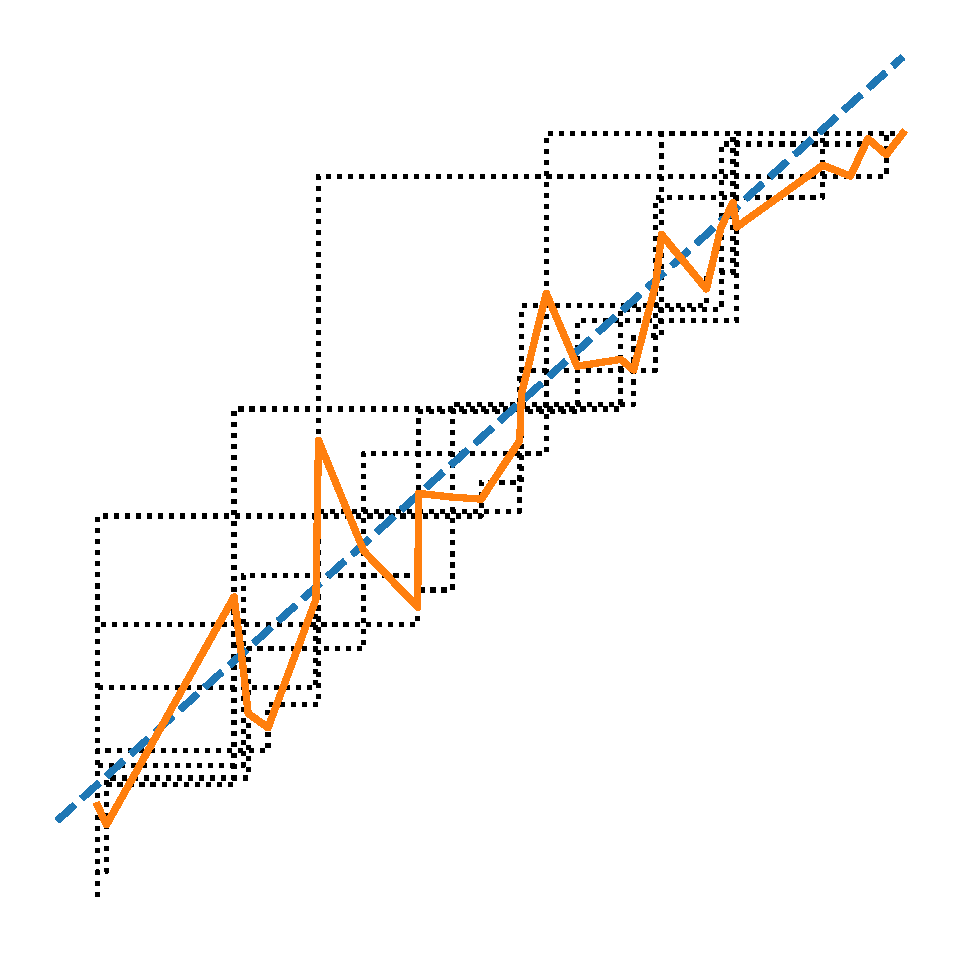
\includegraphics[width=0.4\textwidth]{figures/nonlin/crowd_diagonal}
  \caption{Chacune des frontières de décision en escalier est une mauvaise
    approximation de la vraie frontière qui est la diagonale en trait
    interrompu. Cependant, combiner ces escalier (trait plein) permet une
    meilleure approximation de la diagonale.}
  \label{fig:crowd_diagonal}
\end{figure}


Les méthodes ensemblistes sont particulièrement pertinentes lorsque les modèles
que l'on combine ont été appris par des apprenants faibles, c'est-à-dire
simples à entraîner et peu performants.  En pratique, si les modèles
individuels sont déjà performants et robustes au bruit, le modèle ensembliste
ne sera pas nécessairement meilleur. On utilise le plus souvent des arbres de
décision comme modèles individuels.

\subsection{Bagging} Mais comment créer {\it plusieurs} arbres de décision
différents à partir d'un unique jeu de données ? Le \textbf{bagging} est une
méthode parallèle, basée sur le ré-échantillonnage, qui permet de créer des
arbres indépendants les uns des autres.

Il consiste à former $B$ versions de $\DD$ par \textbf{échantillonnage
  bootstrap}, autrement dit en tirant $n$ exemples de $\DD$ {\it avec
  remplacement}. Ainsi, chaque exemple peut apparaître plusieurs fois, ou pas
du tout, dans $\DD_b$. Chaque arbre est entraîné sur un de ces échantillons
boostrap, ce qui peut être fait en parallèle. Les $B$ prédictions sont ensuite
combinées
\begin{itemize}
\item par vote de la majorité dans le cas d'un problème de classification ; 
\item en prenant la moyenne dans le cas d'un problème de régression.
\end{itemize}

\paragraph{Taille d'un échantillon bootstrap $\bullet$}
La probabilité que $(\xx^i, y^i)$ apparaisse dans $\DD_b$ peut être calculée
comme le complémentaire à 1 de la probabilité que $(\xx^i, y^i)$ ne soit tiré
aucune des $n$ fois. La probabilité de $(\xx^i, y^i)$ soit tiré une fois vaut
$\frac1n$. Ainsi
\begin{equation*}
  \PP[(\xx^i, y^i) \in \DD_b] = 1 - \left(1 - \frac1n\right)^n.
\end{equation*}
Quand $n$ est grand, cette probabilité vaut donc environ
$1 - e^{-1} \approx 0.632$, car la limite en $+\infty$ de
$\left(1 + \frac{x}{n}\right)^n$ vaut $e^x$.  Ainsi, $\DD_b$ contient environ
deux tiers des observations de $\DD$.



\subsection{Forêts aléatoires}
La puissance des méthodes ensemblistes se révèle lorsque les apprenants faibles
sont indépendants conditionnellement aux données, autrement dit aussi
différents les uns des autres que possible, afin que leurs erreurs puissent se
compenser les unes les autres. Pour atteindre cet objectif, l'idée des
\textbf{forêts aléatoires} (ou \textit{random forests}) est de construire les
arbres individuels non seulement sur des échantillons différents (comme pour le
bagging), mais aussi en utilisant des {\it variables} différentes.

Plus précisément, les arbres construits pour former une forêt aléatoire
diffèrent de ceux appris par CART en ce que, à chaque n{\oe}ud, on commence par
sélectionner $q < p$ variables aléatoirement, avant de choisir la variable
séparatrice {\it parmi celles-ci}. En classification, on utilise typiquement
$q \approx \sqrt{p}$, ce qui permet aussi de réduire considérablement les temps
de calculs puisqu'on ne considère que peu de variables à chaque n{\oe}ud (5
pour un problème à 30 variables, 31 pour un problème avec 1000 variables). Pour
la régression, le choix par défaut est plutôt de $q \approx \frac{p}3.$ Ces
valeurs sont basées sur la pratique ; la théorie des forêts aléatoires est
toujours très peu développée, bien que cette méthode ait été proposée il y a
une vingtaine d'années.


\section{Compléments $\bullet \bullet$}

\subsection{Classification binaire avec un perceptron $\bullet \bullet$}
\label{sec:perceptron_binary}
\paragraph{Modèle}
Dans le cas d'un problème de classification binaire, on peut aussi utiliser
directement une fonction de seuil :
\begin{equation}
  \label{eq:seuil}
  f\colon \xx \mapsto 
  \begin{cases}
    0 & \text{ si } o(\xx) \leq 0 \\
    1 & \text{ sinon.}
  \end{cases}
\end{equation}

\paragraph{Fonction de coût} On utilise alors une fonction de coût connue sous
le nom de \textbf{critère du perceptron} :
\begin{equation}
  \label{eq:perceptron}
  L(y^i, f(\xx^i)) = \max(0, - y^i o(\xx^i)) = 
  \max(0, - y^i \innerproduct{\ww,~\xx})
\end{equation}
Ce critère est proche de la fonction d'erreur hinge (voir section 2.2 de la
PC~4). Quand la combinaison linéaire des entrées a le bon signe, le critère du
perceptron est nul. Quand elle a le mauvais signe, le critère du perceptron est
d'autant plus grand que cette combinaison linéaire est éloignée de 0.

\paragraph{Entraînement}
En utilisant ce critère, la règle d'actualisation~\eqref{eq:update_rule}
devient :
\begin{equation*}
  \label{eq:update_rule_binclass}
  w_j \leftarrow \begin{cases}
    0 & \text{ si } y^i o(\xx^i) > 0 \\
    - y^i x_j^i & \text{ sinon.}
  \end{cases}
\end{equation*}
Ainsi, quand le perceptron fait une erreur de prédiction, il déplace la
frontière de décision de sorte à corriger cette erreur.

\subsection{Approximation universelle $\bullet \bullet$}
\label{sec:universal_approx}
\paragraph{Théorème de l'approximation universelle} 
Soit $a\colon \RR \to \RR$ une fonction non constante, bornée, continue et
croissante et $K$ un sous-ensemble compact de $\RR^P$. Étant donné
$\epsilon > 0$ et une fonction $f$ continue sur $K$, il existe un entier $m$,
$m$ scalaires $d_1,d_2, \ldots, d_m$, $m$ scalaires
$b_i, b_2, \ldots, b_m$, et $m$ vecteurs $\ww_1, \ww_2, \ldots, \ww_m$ de
$\RR^p$ tels que pour tout $\xx \in K$,
\begin{equation*}
  \lvert f(\xx) - \sum_{i=1}^m d_i \; a \left( \langle \ww_i, \xx \rangle + 
    b_i \right) \rvert < \epsilon.
\end{equation*}
En d'autres termes, toute fonction continue sur un sous-ensemble compact de
$\RR^p$ peut être approchée avec un degré de précision arbitraire par un
perceptron multi-couche à une couche intermédiaire contenant un nombre fini
de neurones.

  
Ce théorème\footnote{Initialement démontré dans \textit{Approximation by
    superpositions of a sigmoidal function}, G. Cybenko. Mathematics of
  Control, Signals and Systems, 2(4):303--314 (1989) et affiné dans
  \textit{Approximation capabilities of multilayer feedforward networks,}
  K. Hornik, Neural Networks 4(2):241--257 (1991).}  montre la puissance de
modélisation du perceptron multi-couche. Cependant, ce résultat ne nous donne
ni le nombre de neurones qui doivent composer cette couche intermédiaire, ni
les poids de connexion à utiliser. Les réseaux de neurones à une seule couche
cachée sont généralement peu efficaces, et on aura souvent de meilleurs
résultats en pratique avec plus de couches.


\subsection{Rétropropagation $\bullet \bullet$}
\label{sec:backprop}
Pour actualiser le poids de connexion $w^h_{jq}$ du neurone $j$ de la couche
$(h-1)$ vers le neurone $q$ de la couche $h$, nous devons calculer
$\frac{\partial L(y^i, f(\xx^i))}{\partial w^h_{jq}}.$ Pour ce faire, nous
pouvons appliquer le théorème de dérivation des fonctions composées ({\it chain
  rule} en anglais). Nous notons $o^h_j$ la combinaison linéaire des entrées du
$j$-ème neurone de la couche $h$ ; en d'autres termes, $z^h_j =
a_h(o^h_j)$. Par convention, nous considérerons que $z^0_j = x_j$. Ainsi,
\begin{equation}
  \label{eq:mlp_gradient}
  \frac{\partial L(y^i, f(\xx^i))}{\partial o^h_q} 
  \frac{\partial o^h_q}{\partial w^h_{jq}} 
  = \frac{\partial L((y^i, f(\xx^i))}{\partial z^h_q} 
  \frac{\partial z^h_q}{\partial o^h_q} 
  \frac{\partial o^h_q}{\partial w^h_{jq}}   
\end{equation}
et donc   
\begin{equation}
  \begin{split}
    \frac{\partial L(y^i, f(\xx^i))}{\partial w^h_{jq}} & =
    \left(\sum_{r=1}^{p_{h+1}}  \frac{\partial L(y^i, f(\xx^i))}{\partial o^{h+1}_r}  
      \frac{\partial o^{h+1}_r}{\partial z^h_q} \right)
    \frac{\partial z^h_q}{\partial o^h_q} 
    \frac{\partial o^h_q}{\partial w^h_{jq}} \\
    & = \left(\sum_{r=1}^{p_{h+1}}  \frac{\partial L(y^i, f(\xx^i))}{\partial o^{h+1}_r}  
      w^{h+1}_{qr} \right) a_h'(o^h_q) \; z^{h-1}_j.    
  \end{split}
\end{equation}

Le gradient nécessaire à l'actualisation des poids de la couche $h$ se
calcule donc en fonction des gradients
$\frac{\partial L(y^i, f(\xx^i))}{\partial o^{h+1}_r}$ nécessaires pour
actualiser les poids de la couche $(h+1)$.

Cela va nous permettre de simplifier nos calculs en utilisant une technique de
\textbf{mémoïsation}, c'est-à-dire en évitant de recalculer des termes qui
reviennent plusieurs fois dans notre procédure.

Plus précisément, l'entraînement d'un perceptron multi-couche par
\textbf{rétropropagation} consiste à alterner, pour chaque observation
$(\xx^i, y^i)$ traitée, une phase de \textbf{propagation avant} qui permet de
calculer les sorties de chaque neurone, et une phase de
\textbf{rétropropagation des erreurs} dans laquelle on actualise les poids en
partant de ceux allant de la dernière couche intermédiaire vers l'unité de
sortie et en \og remontant \fg~le réseau vers les poids allant de l'entrée vers
la première couche intermédiaire.

\begin{exemple}
  Reprenons le réseau à deux couches intermédiaires décrit sur la
  figure~\ref{fig:mlp}, en utilisant l'identité comme dernière fonction
  d'activation $a_3$, une fonction d'erreur quadratique, et des activations
  logistiques pour $a_1$ et $a_2$. Nous rappelons que la dérivée de la
  fonction logistique peut s'écrire $\sigma'(u) = u' \sigma(u) (1 -
  \sigma(u))$.
  
  Lors de la propagation avant, nous allons effectuer les calculs suivants :
  \begin{align*}
    o^1_q & = \sum_{j=0}^p w_{jq}^1 x_j \; ; \; z^1_q = \sigma(o^1_q) \\
    o^2_q & = \sum_{j=1}^{p_1} w_{jq}^2 z^1_j \; ; \; z^2_q = \sigma(o^2_q) \\
    o^3 & = \sum_{j=1}^{p_2} w^3_j z^2_j \; ; \; f(\xx^i) = z^3 = o^3.
  \end{align*}
  
  Lors de la rétropropagation, nous calculons tout d'abord 
  \begin{equation*}
    \frac{\partial L(y^i, f(\xx^i))}{\partial w^3_j} =      
    \left(f(\xx^i) - y^i \right) \frac{\partial f(\xx^i)}{\partial w^3_j} =
    \left(f(\xx^i) - y^i \right) z^2_j
  \end{equation*}
  en utilisant les valeurs de $f(\xx^i)$ et $z^2_j$ que nous avons mémorisées
  lors de la propagation avant. Ainsi
  \begin{equation*}
    w^3_j \leftarrow w^3_j - \eta \left(f(\xx^i) - y^i \right) z^2_j.
  \end{equation*}
  
  Nous pouvons ensuite appliquer~\ref{eq:mlp_gradient} et calculer 
  \begin{equation*}
    \frac{\partial L(y^i, f(\xx^i))}{\partial w^2_{jq}}  =      
    \frac{\partial L(y^i, f(\xx^i))}{\partial o^2_q} 
    \frac{\partial o^2_q}{\partial w^2_{jq}} 
  \end{equation*}
  où 
  \begin{equation}
    \label{eq:backprop_layer2}
    \frac{\partial L(y^i, f(\xx^i))}{\partial o^2_q} =      
    \frac{\partial L(y^i, f(\xx^i))}{\partial f(\xx^i)} w^3_q \sigma'(o^2_q) = 
    \left(f(\xx^i) - y^i \right) w^3_q z^2_q (1-z^2_q)
  \end{equation}
  et 
  \begin{equation*}
    \frac{\partial o^2_q}{\partial w^2_{jq}} = z^1_j.
  \end{equation*}
  Nous pouvons donc utiliser les valeurs de $f(\xx^i)$, $z^2_q$ et $z^1_j$
  mémorisées lors de la propagation avant, et $w^3_q$ que nous venons
  d'actualiser, pour actualiser $w^2_{jq}$ par
  \begin{equation*}
    w^2_{jq} \leftarrow w^2_{jq} - \eta \left(f(\xx^i) - y^i \right) 
    w^3_q z^2_q (1-z^2_q) \; z^1_j.
  \end{equation*}
  
  Enfin, nous pouvons de nouveau appliquer~\ref{eq:mlp_gradient} et calculer 
  \begin{equation*}
    \frac{\partial L(y^i, f(\xx^i))}{\partial w^1_{jq}} =  
    % \left(\sum_{r=1}^{p_2}  \frac{\partial L(y^i, f(\xx^i))}{\partial o^2_r}  
    %   w^2_{qr} \right) \sigma'(o^1_q) \; x_j = 
    \left(\sum_{r=1}^{p_2}  \frac{\partial L(y^i, f(\xx^i))}{\partial o^2_r}  
      w^2_{qr} \right) z^1_q (1 - z^1_q) \; x_j.
  \end{equation*}
  Encore une fois, nous disposons de tous les éléments nécessaires : $z_q^1$
  a été calculé lors de la propagation avant, les poids $w^2_{qr}$ ont été
  actualisés à l'étape précédente, et les dérivées partielles $\frac{\partial
    L(y^i, f(\xx^i))}{\partial o^2_q}$ ont elles aussi été calculées à
  l'étape précédente (\ref{eq:backprop_layer2}). Nous pouvons donc effectuer
  aisément notre dernière étape de rétropropagation :
  \begin{equation*}
    w^1_{jq} \leftarrow w^1_{jq} - \eta \left(\sum_{r=1}^{p_2}  
      \frac{\partial L(y^i, f(\xx^i))}{\partial o^2_r}  
      w^2_{qr} \right) z^1_q (1 - z^1_q) \; x_j.
  \end{equation*}
\end{exemple}


Il est bien sûr possible d'ajouter une unité de biais à chaque couche intermédiaire
; les dérivations se font alors sur le même principe.


\subsection{Réécriture de la régression ridge $\bullet \bullet$}
\label{sec:ridge_rewrite}

L'expression~\eqref{eq:reg_ridge_beta} peut se réécrire en multipliant à gauche
par $\left( \lambda I_p + X^\top X \right)$, comme
\begin{equation*}
  \bbeta^* = X^\top \aalpha \text{ avec }
  \aalpha = \frac1{\lambda} \left(y - X \bbeta^* \right).
\end{equation*}
Ainsi $\lambda \aalpha = y - X X^\top \aalpha$ et donc 
\begin{equation*}
  \aalpha = \left(\lambda I_n + X X^\top \right)^{-1} y.
\end{equation*}

Ainsi, 
\begin{equation*}
  \langle \xx,  \bbeta^* \rangle = \xx X^\top \aalpha = \xx X^\top (\lambda I_n + XX^\top)^{-1} y.
\end{equation*}



\subsection{Noyau radial gaussien $\bullet \bullet$}
\label{sec:rbf_kernel}
Soit $k$ le noyau radial gaussien de bande passante $\sigma > 0$ sur $\RR^p$ :
\begin{eqnarray*}
  k\colon \RR^p \times \RR^p & \to & \RR \\
  \xx,~\xx^\prime & \mapsto & \exp\left( - \frac{||\xx - \xx^\prime||^2}{2 \sigma^2} \right).
\end{eqnarray*}
Alors
\begin{align*}
  k(\xx, \xx^\prime) & = \exp\left( - \frac{||\xx||^2}{2 \sigma^2} \right)
                 \exp\left( - \frac{\innerproduct{\xx,~\xx^\prime}}{\sigma^2} \right)
                 \exp\left( - \frac{||\xx^\prime||^2}{2 \sigma^2} \right)  \\
               & = \psi(\xx) 
                 \sum_{r=0}^{+ \infty} 
                 \left( - \frac{\innerproduct{\xx,~ \xx^\prime}^r}{\sigma^{2r} r! } \right) \psi(\xx^\prime) 
    = \sum_{r=0}^{+ \infty} 
    \left( - \frac{\innerproduct{\psi(\xx)^{1/r} \xx, \psi(\xx^\prime)^{1/r} \xx^\prime}^r}{\sigma^{2r} r! } \right) 
\end{align*}
avec
$\psi\colon \RR^p \to \RR, \quad \xx \mapsto \exp\left( -\frac{||\xx||^2}{2
    \sigma^2} \right).$ Cela explique pourquoi l'espace de redescription
correspondant à ce noyau est de dimension infinie.

\subsection{Noyaux pour chaînes de caractères $\bullet \bullet$}
\label{sec:more_kernels}
L'astuce du noyau nous permet aussi de travailler sur des données complexes
sans avoir à les exprimer tout d'abord en une représentation vectorielle de
longueur fixe. C'est le cas en particulier pour les données représentées par
des {\it chaînes de caractères,} comme du texte ou des séquences biologiques
telles que de l'ADN (définies sur un alphabet de 4 lettres correspondant aux 4
bases nucléiques) ou des protéines (définies sur un alphabet de 21 acides
aminés.)
  
Étant donné un alphabet $\Acal$, nous utilisons maintenant $\XX = \Acal^*$
(c'est-à-dire l'ensemble des chaînes de caractères définies sur $\Acal$.) La
plupart des noyaux sur $\XX$ sont définis en utilisant l'idée que plus deux
chaînes $x$ et $x'$ ont de sous-chaînes en commun, plus elles sont semblables.
Étant donnée une longueur $k \in \NN$ de sous-chaînes, nous transformons une
chaîne $x$ en un vecteur de longueur $|\Acal|^k$ grâce à l'application
$\phi\colon x \mapsto (\psi_u(x))_{u \in \Acal^k},$ où $\psi_u(x)$ est le nombre
d'occurrences de $u$ dans $x$. $\psi$ peut être modifiée pour permettre les
alignements inexacts, ou autoriser en les pénalisant les « trous » (ou {\it
  gaps}.)
On peut alors définir le noyau pour chaînes de caractères suivant :
\begin{eqnarray*}
  k \colon \Acal^* \times \Acal^* & \to & \RR \\
  x, x^\prime & \mapsto & \sum_{u \in \Acal^k} \psi_u(x) \psi_u(x^\prime).
\end{eqnarray*}

Formellement, ce noyau nécessite de calculer une somme sur $|\Acal^k|$ =
$|\Acal|^k$ termes. Cependant, il peut être calculé de manière bien plus
efficace en itérant uniquement sur les $(|x|+1-k)$ chaînes de longueur $k$
présentes dans $x$, les autres termes de la somme valant nécessairement 0. Il
s'agit alors d'un calcul en $\mathcal{O}(|x| +|x^\prime|)$.

Dans le cas des protéines humaines, si l'on choisit $k=8,$ on remplace
ainsi un calcul dans un espace de redescription de dimension supérieure à
37 milliards ($21^8$) par une somme sur moins de 500 termes (la longueur
moyenne d'une protéine humaine étant de 485 acides aminés.)

\subsection{SVM à noyau $\bullet \bullet$}
\label{sec:kernel_svm}
Reprenons la formulation duale de la SVM à marge souple (à savoir la
formulation donnée à la question 2 de la section 2.2 de la PC~4) :
\begin{align}
  \label{eq:soft-margin-dual-pb}
  \max_{\aalpha \in \RR^n} & 
                           \sum_{i=1}^n  \alpha_i- 
                           \frac{1}{2} \sum_{i=1}^n \sum_{l=1}^n \alpha_i \alpha_l y^i y^l \innerproduct{\xx^i,~\xx^l} \\
  \nonumber \text{ t. q. } & \sum_{i=1}^n \alpha_i y^i = 0 \text{ et }  0 \leq \alpha_i
                             \leq C, \text{ pour tout } i=1, \dots, n.
\end{align}

Posons $k\colon \RR^p \times \RR^p \to \RR$ un noyau, $\HH$ l'espace de
redescription correspondant, et $\phi\colon \RR^p \to \HH$ l'application
telle que pour tout $(\xx, \xx^\prime) \in \RR^p \times \RR^p$, $k(\xx, \xx^\prime) = \innerproduct{\phi(\xx),~\phi(\xx^\prime)}_\HH.$

Apprendre une SVM dans l'espace de redescription $\HH$ (et non pas dans $\RR^p$) revient à résoudre 
\begin{align}
  \label{eq:soft-margin-dual-pb-featspace}
  \max_{\aalpha \in \RR^n} & 
                           \sum_{i=1}^n  \alpha_i- 
                           \frac{1}{2} \sum_{i=1}^n \sum_{l=1}^n \alpha_i \alpha_l y^i y^l \innerproduct{\phi(\xx^i),~\phi(\xx^l)}_\HH \\
  \nonumber \text{ t. q. } & \sum_{i=1}^n \alpha_i y^i = 0 \text{ et }  0 \leq \alpha_i
                             \leq C, \text{ pour tout } i=1, \dots, n.
\end{align}

qui est donc équivalent à résoudre
\begin{align}
  \label{eq:kernel-svm-dual-pb}
  \max_{\aalpha \in \RR^n} & 
                           \sum_{i=1}^n  \alpha_i- 
                           \frac{1}{2} \sum_{i=1}^n \sum_{l=1}^n \alpha_i \alpha_l y^i y^l k(\xx^i,~\xx^l) \\
  \nonumber \text{ t. q. } & \sum_{i=1}^n \alpha_i y^i = 0 \text{ et }  0 \leq \alpha_i
                             \leq C, \text{ pour tout } i=1, \dots, n.
\end{align}

Remarquez que l'on cherche toujours seulement $n$ coefficients ! C'est ce qui
fait la force des SVM à noyaux : on peut apprendre des modèles plus complexes
sans changer le nombre de paramètres à apprendre, autrement dit sans augmenter
le temps de calcul. Attention, ce temps de calcul dépend maintenant du nombre
d'observations, qui peut être très élevé à l'ère du Big Data...

Enfin, la fonction de décision est donnée dans le cas linéaire par
$  f\colon \xx \mapsto \innerproduct{\ww, \xx} + b$ et 
peut être réécrite comme 
\begin{equation*}
  f\colon \xx \mapsto \sum_{i=1}^n \alpha_i^* y^i \innerproduct{\xx^i, \xx} + b,
\end{equation*}
d'après la correspondance entre $\ww$ et $\alpha$ donnée dans cette même
question 2 de la partie 2.2 de la PC~4, à savoir
% \begin{equation*}
$\ww^* = \sum_{i=1}^n \alpha_i^* y^i \xx^i.$
% \end{equation*}

Dans le cas à noyau, la fonction de décision est donc donnée par 
\begin{equation*}
  f\colon \xx \mapsto \sum_{i=1}^n \alpha_i^* y^i k(\xx^i, \xx) + b.
\end{equation*}

\subsection{Comment faire pousser un arbre de décision (cas général) $\bullet \bullet$}
\label{sec:grow_tree}
Dans le cas où la variable de séparation est une variable {\it discrète}
pouvant prendre plus de deux valeurs (ou modalités), elle s'accompagne alors
d'un sous-ensemble de ces valeurs $\Scal \subset \text{dom}(x_j).$ Les deux
régions sont
\begin{equation*}
  R_l(j, \Scal) = \{\xx~|~x_j \in \Scal\} ; \hspace{2em} 
  R_r(j, \Scal) = \{\xx~|~x_j \notin  \Scal\}.
\end{equation*}

Dans le cas où la variable de séparation est une variable {\it réelle},
elle s'accompagne alors d'un \textbf{point de séparation} ({\it splitting
  point}) $s$ qui est la valeur de la variable par rapport à laquelle va se
faire la décision. Les deux régions sont alors
\begin{equation*}
  R_l(j, s) = \{\xx~|~x_j < s\} ; \hspace{2em} R_r(j, s) = \{\xx~|~x_j \geq s\}.
\end{equation*}
Si l'on suppose les valeurs prises par la variable $j$ dans $\DD$ ordonnées :
$x_j^1 \leq x_j^2 \leq \dots, \leq x_j^n$, alors les valeurs possibles de $s$
sont $\frac{x^{i+1}_j - x^i_j}2$ pour toutes les valeurs de $i$ telles que
$x^{i+1}_j \neq x^i_j.$


À chaque itération de l'algorithme CART, on itère sur toutes les valeurs
possibles de $j$ et, le cas échéant, toutes les valeurs possibles de $s$ ou
$\Scal$ pour déterminer celle qui minimise localement l'erreur faite en
attribuant à toutes les observations de la région de gauche $(R_l)$ (resp. de
droite $(R_r)$) leur étiquette majoritaire (dans le cas d'un problème de
classification) ou moyenne (dans le cas d'un problème de régression).


Formellement, notons $\Ical$ l'ensemble des variables de
séparations possibles, à savoir l'union
\begin{itemize}
\item des indices $j$ des variables binaires ;
\item des couples $(j, \Scal)$ de paires de variables discrètes à plus de deux
  modalités, et de tous les sous-ensembles $\Scal$ possible de ces modalités ;
\item des couples $(j, s)$ de paires de variables continues et des points de
  séparation possibles.
\end{itemize}
Nous noterons donc ainsi $\zeta \in \Ical$ une variable de séparation,
accompagnée si elle est discrète d'un sous-ensemble $\Scal$ de valeurs ou si
elle est continue d'un seuil $s$, ce qui nous permet de noter $R_l(\zeta)$ et
$R_r(\zeta)$ les deux régions définies par $\zeta$ indépendamment de sa nature
binaire, discrète ou continue.

Notons maintenant
\begin{equation*}
  y_l(\zeta) =
  \begin{cases}
    \argmax_{c \in \{0, 1\}} \abs{\{i:\xx^i \in R_l(\zeta) ~|~y^i=c\}} & \text{ pour un problème de classification binaire } \\
    \frac1{\abs{\{i:\xx^i \in R_l(\zeta)\}}} \sum_{i:\xx^i \in R_l(\zeta)} y^i & \text{ pour un problème de régression.}
  \end{cases}
\end{equation*}

on généralise alors l'équation~\eqref{eq:erm_binary_tree} en :
\begin{equation}
  \argmin_{\zeta \in \Ical} \left( 
    \frac1{\abs{R_l(\zeta)}} \sum_{i: \xx^i \in R_l(\zeta)} L(y^i, y_l(\zeta))  + 
     \frac1{\abs{R_r(\zeta)}} \sum_{i: \xx^i \in R_r(\zeta)} L(y^i, y_r(\zeta))
  \right)
\end{equation}

Dans le cas d'un problème de régression, la fonction de perte $L$ est, encore
une fois, l'erreur quadratique moyenne. Voir la section~\ref{sec:impurity} pour
les problèmes de classification.

Ainsi, avec beaucoup d'échantillons et beaucoup de variables continues, un
arbre de décision peut être long à entraîner : il faut à chaque n{\oe}ud tester
toutes les variables et chacun de leur seuils, ce qui fait de l'ordre de $np$
opérations par n{\oe}ud.

\subsection{Critères d'impureté pour les arbres de décision $\bullet \bullet$}
\label{sec:impurity}
Dans le cas d'un problème de classification, on appelle la fonction de perte
utilisée pour apprendre un arbre de décision son \textbf{critère d'impureté} :
il quantifie à quel point la région considérée est \og polluée \fg~par des
éléments des classes qui n'y sont pas
majoritaires.

Il existe plusieurs critères d'impureté, que nous détaillons dans cette section
: l'\textbf{erreur de classification}, l'\textbf{entropie croisée} et
l'\textbf{impureté de Gini}. Pour les définir, nous allons utiliser la notation
$p_c(R)$ pour indiquer la proportion d'exemples d'entraînement de la région $R$
qui appartiennent à la classe $c$ :
\begin{equation*}
  p_c(R) = \frac1{\lvert R \rvert} \sum_{i : \xx^i \in R} \delta(y^i, c).       
\end{equation*}

L'\textbf{erreur de classification} définit l'impureté
d'une région $R$ comme la proportion d'individus de cette région qui
n'appartiennent pas à la classe majoritaire :
\begin{equation}
  \label{eq:impurity_error}
  \text{Imp}(R) = 1 - \max (p_0(R),~p_1(R)).
\end{equation}
Si tous les individus de $R$ appartiennent à la même classe, l'erreur de
classification vaut $0$ ; à l'inverse, si $R$ contient autant d'exemples de
chacune des 2 classes, $p_0(R) \approx \frac12$ quelle que soit la classe
$c$, et l'erreur de classification vaut $\frac12.$

L'\textbf{entropie croisée} définit l'impureté d'une région $R$ de
sorte à choisir la séparation qui maximise le gain d'information : le but de la
construction est alors de minimiser la quantité d'information supplémentaire
nécessaire pour étiqueter correctement les exemples d'entraînement de $R$.
\begin{equation}
  \label{eq:impurity_entropy}
  \text{Imp}(R) = - \left(p_0(R) \log_2 p_0(R) + p_1(R) \log_2 p_1(R)\right).
\end{equation}
Si tous les exemples d'une région appartiennent à la même classe, l'entropie
croisée de cette région vaut $0$ ; à l'inverse, si une région contient autant
d'exemples de chacune des 2 classes, l'entropie croisée vaut $\log_2(2)=1.$
  
Enfin, la définition la plus utilisée de l'impureté est l'\textbf{impureté de
  Gini}, qui permet de quantifier la probabilité qu'une observation du jeu
d'entraînement soit mal étiquetée si elle était étiquetée aléatoirement en
fonction de la distribution des étiquettes dans $R$ :
\begin{equation*}
  \text{Imp}(R) = p_0(R) \left(1 - p_0(R)\right) + p_1(R) \left(1 - p_1(R)\right).
\end{equation*}
Si tous les exemples de $R$ appartiennent à la même classe, l'impureté de
Gini de $R$ vaut $0$ ; à l'inverse, si une région contient autant
d'exemples de chacune des 2 classes, l'impureté de Gini vaut $\frac12.$ 




\begin{plusloin}
\item Plusieurs cours de 2A et 3A aux Mines traitent d'apprentissage profond et
  de machine learning non-linéaire.
\item Nous n'avons dans ce chapitre qu'esquissé les briques de bases du
  \textit{deep learning.} Pour aller plus loin, plongez-vous dans
  \href{http://www.deeplearningbook.org}{\textit{Deep learning} de
    I. Goodfellow, Y. Bengio et A. Courville (2016)} ou visitez
    \href{http://playground.tensorflow.org/}{http://playground.tensorflow.org/}
    pour jouer avec
  l'architecture et l'entraînement d'un réseau de neurones profond.
\item Le domaine des méthodes à noyaux est très vaste. De nombreux ouvrages ont
  été dédiés au sujet, en particulier \textit{Learning with Kernels: Support
    Vector Machines, Regularization, Optimization, and Beyond}, B. Schölkopf et
  A.~J. Smola (2002).
\item Une autre façon de construire plusieurs apprenants faibles à partir du
  même jeu de données est le \textbf{boosting}, 
  dans lequel chaque nouvel apprenant est construit en fonction des
  performances du précédent. Le \textbf{boosting de gradient}, ou GBOOST, en est
  l'exemple le plus populaire.
\end{plusloin}

%-*- coding: utf-8 -*-
\section{QCM}
\paragraph{Question 1.} Vous disposez d'un jeu de données contenant un millier
d'observations. Les performances des modèles linéaires que vous avez essayés ne
sont pas satisfaisantes. Vous décidez d'utiliser un réseau de neurones
artificiels. Vaut-il mieux essayer
\begin{itemize}
\item[$\square$] un perceptron ;
\item[$\square$] un perceptron multi-couche avec une couche intermédiaire d'une dizaine de neurones ;
\item[$\square$] un perceptron multi-couche avec 4 couches intermédiaires d'une centaine de neurones chacune ?
\end{itemize}

\paragraph{Question 2.} La qualité du modèle appris par un réseau de neurones artificiel dépend
\begin{itemize}
\item[$\square$] de l'architecture de ce réseau ;
\item[$\square$] des fonctions d'activations ;
\item[$\square$] de la vitesse d'apprentissage (c'est-à-dire le pas de la descente de gradient) ;
\item[$\square$] de la quantité de données utilisées. 
\end{itemize}

\paragraph{Question 3.} L'astuce du noyau s'applique
\begin{itemize}
\item[$\square$] à la régression ridge ;
\item[$\square$] à la régression lasso ;
\item[$\square$] aux arbres de décision.
\end{itemize}

\paragraph{Question 4.} Considérons un arbre de décision appris sur un jeu de
données contenant $n$ observations décrites par $p$ variables. Sa profondeur
est au plus
\begin{itemize}
\item[$\square$] $p$.
\item[$\square$] $\log_2(p)$.
\item[$\square$] $n$.
\item[$\square$] $\log_2(n)$.
\item[$\square$] $\min(n, p)$.
\item[$\square$] $\min(\log_2(n), \log_2(p))$.
\end{itemize}

\paragraph{Question 5.} Le bagging permet de
\begin{itemize}
\item[$\square$] Combiner plusieurs jeux de données en un seul pour créer un meilleur modèle.
\item[$\square$] Créer plusieurs jeux de données à partir d'un seul, en sélectionnant aléatoirement les observations.
\item[$\square$] Créer plusieurs jeux de données à partir d'un seul, en sélectionnant aléatoirement les variables.
\item[$\square$] Combiner plusieurs modèles simples en un meilleur modèle.
\end{itemize}


\section*{Solution}
{%
\noindent
\rotatebox[origin=c]{180}{%
\noindent
\begin{minipage}[t]{\linewidth}
\paragraph{Question 1.}  Le perceptron est un modèle linéaire, il n'aura pas
une meilleure performance. Le perceptron multi-couche avec 4 couches
intermédiaires d'une centaine de neurones chacune contient beaucoup de
paramètres pour 1\,000 observations seulement et risque de surapprendre. \newline

\paragraph{Question 2.} Toutes les réponses sont valides. \newline

\paragraph{Question 3.} Ni le lasso (à cause de la norme $\ell_1$) ni les
arbres de décision (non paramétriques) ne peuvent s'écrire en faisant
apparaitre les observations uniquement au sein de produits scalaires entre
observations. Seule la régression ridge est donc \textit{kernelizable}. \newline

\paragraph{Question 4.} Dans le pire des cas, chaque niveau de l'arbre de
décision met un seul échantillon dans la branche de gauche, et tous les autres
dans la branche de droite. On obtient donc une profondeur de $n$. \newline

\paragraph{Question 5.} Le bagging consiste à créer plusieurs jeux de données à
partir d'un seul, en sélectionnant aléatoirement les observations, afin de
créer autant de modèles simples combinés en un modèle robuste.
\end{minipage}%
}%


%%% Local Variables:
%%% mode: latex
%%% TeX-master: "../../sdd_2025_poly"
%%% End:



%%% Local Variables:
%%% mode: latex
%%% TeX-master: "../sdd_2025_poly"
%%% End:

